\chapter{Decoupling della fase ascendente e fase discendente}\label{chapter:decoupling}

Nel capitolo precedente abbiamo visto come si può usare l'interpretazione astratta per l'analisi statica di un programma. Il metodo proposto si compone di una astrazione del dominio concreto, quindi una connessione di Galois \(\mathbb{C}\galois{\alpha}{\gamma}\mathbb{A}\),  ed un sistema di equazioni  astratte \(F_{\mathbb{A}}\) che correttamente approssimano il comportamento del programma. Il calcolo avviene poi in due fasi, una prima fase, detta ascendente, che calcola un post-fix-point di \(F_{\mathbb{A}}\) in cui si utilizza un estrapolatore (come il widening) per assicurare la convergenza seguita da una fase discendente che ne migliora i risultati. Va notato che entrambi le fasi vengono eseguite sullo stesso dominio \(\mathbb{A}\).

L'idea proposta in \cite{DBLP:conf/aplas/ArceriMZ22} è quella di disaccoppiare (decouple) le due fasi, ovvero di calcolare la fase discendente su un dominio diverso, e più preciso, rispetto a quello della fase ascendente. L'obbiettivo è quello di ottenere una analisi più precisa senza pagare il costo in termini di efficienza del calcolare la fase ascendente con un dominio molto preciso. In più la fase discendente può essere stoppata dopo un qualsiasi numero di iterazioni e comunque fornire un risultato corretto. Per questo può essere più facile ottenere un buon tradeoff tra precisione ed efficienza.

La notazione che verrà usata per indicare questo approccio decoupled all'interpretazione astratta è \(\mathbb{A}\uparrow\downarrow\mathbb{D}\), dove \(\mathbb{A}\) è il dominio astratta usato nella fase ascendente e \(\mathbb{D}\) è quello utilizzato nella fase discendente. Con questo metodo avremo bisogno di una doppia connessione di Galois in questo modo \(\mathbb{C}\galois{\alpha_{\mathbb{A}}}{\gamma_{\mathbb{D}}}\mathbb{D}\galois{\alpha_{\mathbb{D}\uparrow\downarrow\mathbb{D}}}{\gamma_{\mathbb{A}\uparrow\downarrow\mathbb{D}}}\mathbb{A}\) ed è richiesto che la funzione di concretizzazione \(\gamma_{\mathbb{A}\uparrow\downarrow\mathbb{D}}\) sia calcolabile. L'approccio decoupled è graficamente rappresentato nella figura \ref{fig:decFig}. Avendo un sistema di equazioni concrete \(F_{\mathbb{C}}\) correttamente approssimato dal sistema di equazioni \(F_{\mathbb{D}}\) sul dominio \(\mathbb{D}\), e queste ultime ulteriormente approssimate da \(F_{\mathbb{A}}\) sul dominio \(\mathbb{A}\), possiamo riassumere i passaggi del metodo decoupled in questo modo: (1) nella fase ascendente calcoliamo il post-fixpoint \(x^{\nabla}_{\mathbb{A}}\in\mathbb{A}\) di \(F^{\nabla}_{\mathbb{A}}\) con il widening, (2) poi trasferiamo \(x^{\nabla}_{\mathbb{A}}\) nel dominio più preciso \(\mathbb{D}\) tramite la funzione concretizzante \(\gamma_{\mathbb{A}\uparrow\downarrow\mathbb{D}}\), (3) ed infine nella fase discendente si calcola un post-fix-point migliorato \(x^{\Delta}_{\mathbb{D}}\in\mathbb{D}\) usando il sistema di equazioni \(F^{\Delta}_{\mathbb{D}}\) con narrowing partendo da  \(\gamma_{\mathbb{A}\uparrow\downarrow\mathbb{D}}(x^{\nabla}_{\mathbb{A}})\).

\begin{figure}[H]
\centering
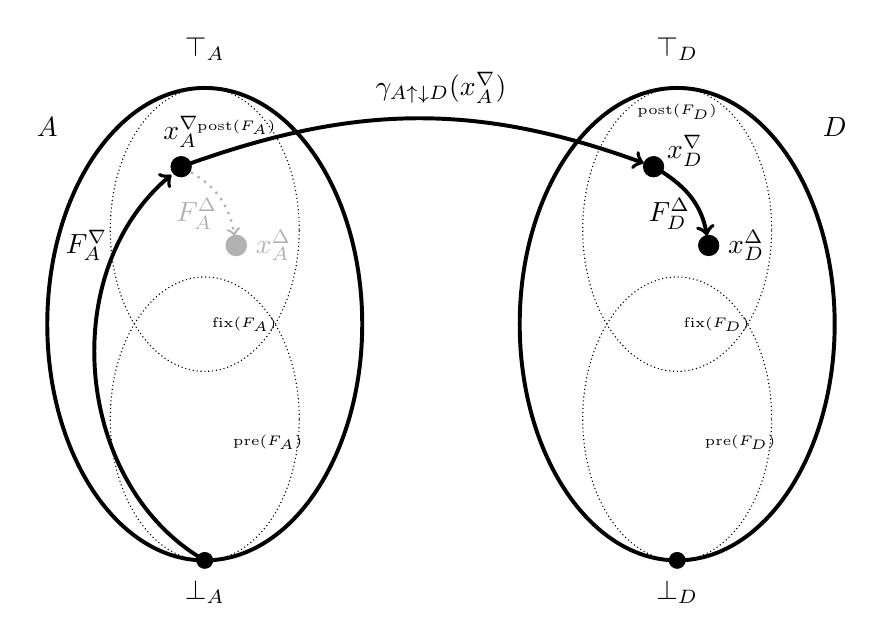
\begin{tikzpicture}
    \draw [line width=0.5mm] (-3, 0) ellipse (2cm and 3cm);
    \draw [line width=0.5mm] (3, 0) ellipse (2cm and 3cm);
    
    \node (top) at (-3, 3.5) {$\top_{\mathbb{A}}$};
    \node (bottom) at (-3, -3.4) {$\perp_{\mathbb{A}}$};
    \node (top) at (3, 3.5) {$\top_{\mathbb{D}}$};
    \node (bottom) at (3, -3.4) {$\perp_{\mathbb{D}}$};
    
    \draw [densely dotted] (-3, -1.2) ellipse (1.2cm and 1.8cm);
    \draw [densely dotted] (-3, 1.2) ellipse (1.2cm and 1.8cm);
    \draw [densely dotted] (3, -1.2) ellipse (1.2cm and 1.8cm);
    \draw [densely dotted] (3, 1.2) ellipse (1.2cm and 1.8cm);
    
    \node (domain) at (-5, 2.5) {\(\mathbb{A}\)};
    \node (domain) at (5, 2.5) {\(\mathbb{D}\)};
    
    \node (bottomStartA) at (-3, -3) {};
    \draw [fill=black] (-3, -3) circle (0.1cm);
    \node (bottomStartD) at (3, -3) {};
    \draw [fill=black] (3, -3) circle (0.1cm);

    \node (pre) at (-2.2, -1.5)  {\tiny pre($F_{\mathbb{A}}$)};
    \node (post) at (-2.6, 2.5)  {\tiny post($F_{\mathbb{A}}$)};
    \node (fix) at (-2.5, 0)  {\tiny fix($F_{\mathbb{A}}$)};
    \node (pre) at (3.8, -1.5)  {\tiny pre($F_{\mathbb{D}}$)};
    \node (post) at (3, 2.7)  {\tiny post($F_{\mathbb{D}}$)};
    \node (fix) at (3.5, 0)  {\tiny fix($F_{\mathbb{D}}$)};
    
    \node [label=above:{$x^{\nabla}_{\mathbb{A}}$}] (widPostA) at (-3.3, 2) {};
    \draw [fill=black, line width=0.1mm] (-3.3, 2) circle (0.13cm);
    \node (widPostD) at (2.7, 2) {};
    \node (widPostDlabel) at (3.1, 2.2) {$x^{\nabla}_{\mathbb{D}}$};
    \draw [fill=black, line width=0.1mm] (2.7, 2) circle (0.13cm);

    \node (fnablaA) at (-4.5, 1) {\(F^{\nabla}_{\mathbb{A}}\)};
    \node (fDeltaA) at (-3.1, 1.4) {\color{black!30}\(F^{\Delta}_{\mathbb{A}}\)};
    \node (fDeltaD) at (2.9, 1.4) {\(F^{\Delta}_{\mathbb{D}}\)};

    \node (concret) at (0, 3) {\(\gamma_{\mathbb{A}\uparrow\downarrow\mathbb{D}}(x^{\nabla}_{\mathbb{A}})\)};
    
    \node [label=right:{\color{black!30}$x^{\Delta}_{\mathbb{A}}$}] (narrPostA) at (-2.6, 1) {};
    \draw [black!30, fill=black!30] (-2.6, 1) circle (0.13cm);
    \node [label=right:{$x^{\Delta}_{\mathbb{D}}$}] (narrPostD) at (3.4, 1) {};
    \draw [fill=black, line width=0.1mm] (3.4, 1) circle (0.13cm);

    \draw[->, line width=0.5mm] (bottomStartA.center) to [out=150, in=220] (widPostA);

    \draw[->, line width=0.3mm, dotted, black!30] (widPostA) to [out=330, in=100] (narrPostA);
    
    \draw[->, line width=0.5mm] (widPostD.center) to [out=330, in=100] (narrPostD);
    \draw[->, line width=0.5mm] (widPostA.center) to [out=20, in=160] (widPostD);
\end{tikzpicture}
    \centering
    \caption{Fase ascendente e discendente disaccoppiate sui domini \(\mathbb{A}\) e \(\mathbb{D}\))}
    \label{fig:decFig}
\end{figure}

\begin{example}
Riprendiamo l'esempio \ref{ex:esempio2} e utilizziamo il dominio decoupled \(\textrm{Sign}\uparrow\downarrow\textrm{Int}\) per cercare una approssimazione della collecting semantics del programma. La funzione concretizzante \(\gamma_{\textrm{Sign}\uparrow\downarrow\textrm{Int}}\) la abbiamo definita nell'esempio \ref{ex:galoisSignInt}. I risultati dell'analisi sono mostrati nella tabella in figura \ref{fig:risDecSingInt}. 

\begin{table}[H]
\begin{minipage}{\textwidth}
    \centering
    \vspace{1cm}
        \[
        \begin{tabular}{|c|c|c|c||c||c|c|c||}
        \hline
        \multicolumn{2}{|c|}{fase} & 
        \multicolumn{2}{c||}{\textbf{ascendente}} & 
        \multicolumn{1}{c||}{\textbf{decoupling}} & 
        \multicolumn{2}{c|}{\textbf{discendente}}\\
        
        \hline 
        \rule{0pt}{14pt} N & WP & 1st & 2nd=\(x^{\nabla}_{\textrm{Sign}}\) & 
        \(\gamma_{\textrm{Sign}\uparrow\downarrow\textrm{Int}}(x^{\nabla}_{\textrm{Sign}})\)& 
        1st & 2nd=\(x^{\Delta}_{\textrm{Int}}\)  \\
        \hline
        $x_1$ &  &  
            $\top_{\textrm{Sign}}$ & $\top_{\textrm{Sign}}$ & 
            $\top_{\textrm{Int}}$ & 
            $\top_{\textrm{Int}}$ & $\top_{\textrm{Int}}$ \\
        \hline
        $x_2$ &  & 
            0 & 0+ & 
            $\left[0, +\infty \right]$ & 
            $\left[0, +\infty \right]$ & $\left[0, 109\right]$ \\
        \hline
        $x_3$ & \checkmark & 
            0 & 0+ & 
            $\left[0, +\infty \right]$ & 
            $\left[0, 99\right]$ & $\left[0, 99\right]$ \\
        \hline
        $x_4$ &  & 
            0 & 0+ & 
            $\left[0, +\infty\right]$ & 
            $\left[0, 49\right]$ & $\left[0, 49\right]$ \\
        \hline
        $x_5$ &  & 
            $\perp_{\textrm{Sign}}$ & + & 
            $\left[1, +\infty \right]$ & 
            $\left[50, 99\right]$ & $\left[50, 99\right]$ \\
        \hline
        $x_6$ &  & 
            $\perp_{\textrm{Sign}}$ & + & 
            $\left[1, +\infty \right]$ & 
            $\left[100, +\infty \right]$ & $\left[100, 109\right]$ \\
        \hline
        \end{tabular}
        \]
    \end{minipage}
    \caption{tabella dei risultati del dominio \(\textrm{Sign}\uparrow\downarrow\textrm{Int}\) divisi per step e fase.}
    \label{fig:risDecSingInt}
\end{table}
\end{example}

\begin{example}
Sempre per il programma dell'esempio \ref{ex:esempio2}, possiamo utilizzare il dominio decoupled \(\textrm{Int}\uparrow\downarrow\widehat{\textrm{Int}}\), dove \(\widehat{\textrm{Int}}\) è il dominio dei sottoinsiemi non ridondanti di Int.
\end{example}